%The data needs to be rich and from real-world apps and projects which justify the use of cases. The research also had to engage with Industry and take a case-based approach situated in real projects. 

\julian{Interim actions:
\begin{enumerate}
    \itemsep0em
    \item (done) Map the methods to the six perspectives in Figure~\ref{fig:six-perspectives-in-the-methodology}. 
    \item Mapping of perspectives into the data that drives them - justify the evidence that each perspective would need.
    \item Data collection methods that will deliver the evidence: I now have the foundation for the rich data I want to collect.
\end{enumerate}}

% Data needed - justify the use of cases
% Therefore...
% Data I am seeking
% Map the data onto the analysis


%This approach is consistent with the traits of qualitative research elegantly summarised in \citealp[pp 113-114]{zieris2020_phd_qualitative_analysis_of_knowledge_transfer_in_pair_programming} that also aligns with and reflects many of the 10 features in \citealt[p.150]{ball2000_putting_ethnography_to_work_cognitive_ethnography}. (Trying to understand things in context)

%To a certain extent, experiments were natural as they arose \textit{in situ} where and when situations arose that were reported by mobile analytics that the development team chose to respond to. \textit{``A key feature of natural experiments is that they offer insight into causal processes, which is one reason why they have an established role in developmental science."}~\citep[p.877]{salkind_encyclopedia_2021_natural_experiment}



%(\textit{c.f.} targeted observation / vectored research~\footnote{MUST-DO ask Marian for her reference on using vectors in questioning. Source: `Petre 2008 Targeted observation of expert software designers. NSF workshop on studying design creativity (Aix-en-Provence, France, February)'})

%`\textbf{Sensebuilding}' methods built on insights found through sense-making, both investigating detail through micro-experiments (i.e., local app experiments) and identifying characteristics and patterns (i.e., macro-discoveries) that were not present in individual case studies (through across-case comparisons).

%\textit{Micro-experiments} (i.e., local app experiments) were created by developing small mobile apps intended to exercise particular aspects of mobile analytics (similar to the `invent the future' adage~\footnote{For example: \url{https://quoteinvestigator.com/2012/09/27/invent-the-future/}}). The inputs to an app were directed in order to determine the outputs from mobile analytics. These helped to answer questions and gaps observed as part of sensemaking.  The local app experiments gave insight into the relationships between tools, quality of analytics, and potential impact of analytics use on apps (i.e., perspectives \uartefacts, \utools, \iartefacts, \itools). 

%\textit{Across-case comparisons} were concerned largely with understanding current practice and identifying potential improvements to practice (i.e., perspectives \uuse and \iuse), as well as the influence of the quality of tools in practice (\itools).


\begin{comment}
Commented out after adding the grouping suggested with Marian on \nth{22} Oct 2021. Preserved until this chapter is in better shape.

\julian{Conflations: 1) data collection methods and analysis 2) contributors and goals also conflated. Action: Group rows by what I was targeting: I need to provide the rationale for the methods I used.} Two suggested groupings to try:
\begin{itemize}
    \item 3 Groupings: Tool outputs, validation, action research. 
    \item 4 Groupings: beacons-and-drill-downs, comparisons, contextualisation and clarification, evaluation through action research.
\end{itemize}
\end{comment}


\section{Text-based methodology maps (a w-i-p)}
\emph{The following hierarchical lists are a work-in-progress while the details are established. They will be replaced and retired.}


{\footnotesize
\begin{description}
    \itemsep0em
    \item[Research Method] :
        \begin{itemize}
            \item Case Study
        \end{itemize}
    \item[Research Tools] :
    \begin{itemize}
        \itemsep0em
        %\item[]
        \item Action Research
        \item[$\bullet$] [Semi-] Controlled Experiment (Field experiments)
        \item Hackathon
    \end{itemize}
    \item[Analytics Provider] :
        \begin{itemize}
            \item Google Play Console with Android Vitals
        \end{itemize}
    \captionof{methodology-map}{Kiwix case study methodology map}
    \label{methodology-map-kiwix-case-study}    
\end{description}
}
% Thanks to https://fedoramagazine.org/latex-typesetting-part-1/ for helping me discover {description} and for enabling me to find workarounds when it didn't render as I'd expected e.g. where I needed to add [$\bullet$] to stop it interpreting [Semi-] as a style.

{\footnotesize
\begin{description}
    \itemsep0em
    \item[Research  Method] :
        \begin{itemize}
            \item Inductive analysis of source code
        \end{itemize}
    \item[Research Tool] TBC
    \item[Data Analysis Method] TBC
    \captionof{methodology-map}{Logging using Mobile Analytics}
    \label{methodology-map-logging-using-mobile-analytics}
\end{description}
}


\begin{comment}
Therefore the research methodology has three main prongs:

\begin{enumerate}
    \itemsep0em
    \item Case-studies: to engage effectively with the organisation, projects, and project teams. The case studies are the source of much of the evidence used in how mobile analytics is used by development teams in practice. See page \pageref{section-case-study-procedure} for details of the case study procedure; \textit{i.e.} the structure of a case study within the context of this research. 
    \item Data-collection: to collect data in practice given the nature of the engagements between research and the projects.
    \item Analysis: to make sense of the manifold rich data sources and the findings that emerge. 
\end{enumerate}

The methodology also includes validation findings and analysis with the development teams who participate in the research. 


\subsection{Rationale}
The rationale for the choice of methods

\newthought{How the methods fit in a framework of theories and complement each other}
\isabel{I would say that the methodology is a description not only of the methods, but also of the rationale for the choice of methods and also how they fit together in a framework of theories, and how they complement and add to each other to provide triangulation and to mitigate threats to validity. So quite a lot to do here.}

\end{comment}


\section{Sources}
\emph{These are interim notes and unlikely to be part of the final version of this chapter.}

\subsection{On Methodology}
\begin{itemize}
    \item \emph{``A Student's Guide to Methodology"}~\citep{clough2012_students_guide_to_methodology}.
    \item \emph{``Creating a wider audience for action research: Learning from case-study research"}~\citep{blichfeldt2006creating}. Online edition available at~\url{http://jrp.icaap.org/index.php/jrp/article/view/23/43}.
    \item \emph{``Action research or case study?"} \url{https://www.nicole-brown.co.uk/action-research-or-case-study/}
    \item \emph{``A gentle guide to research methods"}~\citep{rugg2006_gentle_guide_to_research_methods}.
    \item \emph{``Stepping Stones to Achieving your Doctorate"}~\citep{trafford2008_stepping_stones_to_achieving_your_doctorate}.
    \item \emph{``The How To of Qualitative Research: Strategies for Executing High Quality Projects"}~\citep{aurini2016_how_to_of_qualitative_research}.
    \item \emph{``Empirical Research Methods in Software Engineering"}~\citep{Wohlin2003_empirical_research_methods_in_software_engineering} \textbf{This is one of the key papers to provide support and evidence for using empirical research methods in my research.}
    \item \emph{``Evaluation and Measurement of Software Process Improvement—A Systematic Literature Review"}~\citep{unterkalmsteiner2012_evaluation_and_measurement_of_spi_a_slr}
    \begin{itemize}
        \item ``evaluation strategies were identified, wherein the most common one, “Pre-Post Comparison,” was applied in 49 percent of the inspected papers. Quality was the most measured attribute (62 percent)"
        \item ``CONCLUSION-The evaluation validity of SPI initiatives is challenged by the scarce consideration of potential confounding factors, particularly given that “Pre-Post Comparison” was identified as the most common evaluation strategy, and the inaccurate descriptions of the evaluation context. Measurements to assess the short and mid-term impact of SPI initiatives prevail, whereas long-term measurements in terms of customer satisfaction and return on investment tend to be less used."
    \end{itemize}
    \item \emph{``Grounded theory in software engineering research: a critical review and guidelines"} \url{https://doi.org/10.1145/2884781.2884833} if I decide to wade into grounded theory... (I aim not to).
\end{itemize}

%\isabel{Next call, 2 hours on Thursday 9th Sept 09:30 - 11:30 - Whiteboarding session.}

\section{Placeholders}
\begin{itemize}
    \item \citep{soiferman2010_compare_and_contrast_inductive_and_deductive_research_approaches}
\end{itemize}

\section*{Preamble - what needs doing to craft this chapter}
{\small
Recap what I found in the Literature Review, to validate the RQs. Then start with the RQs to consider how they can be answered in the research. Highlight the value and relevance of evaluating this in practice. Add `in practice' to my RQ. Look at literature on the theory of generalisation from case studies - Ask Marian for advice on this.

Determine what's needed to answer each sub-question and the methods needed to answer them. Formulate hypotheses from the RQ's - consider first falsifying the null hypothesis. Pointers: the research onion - Saunders, appeals to logic, appeal to authority - prior practice, what are the threats to validity, maintain the methods developers use which is outside the scope of this chapter,

Create a diagram to map out the connections between the case studies and the evidence they provide. Show the dependencies between the RQs and the case studies and the evidence they provide.

Arosha suggested a layered diagram with evidence at the base. or perhaps something akin to Akshika's diagram~\ref{fig:akshikas-methodologies-map}.
}

\begin{figure}
    \centering
    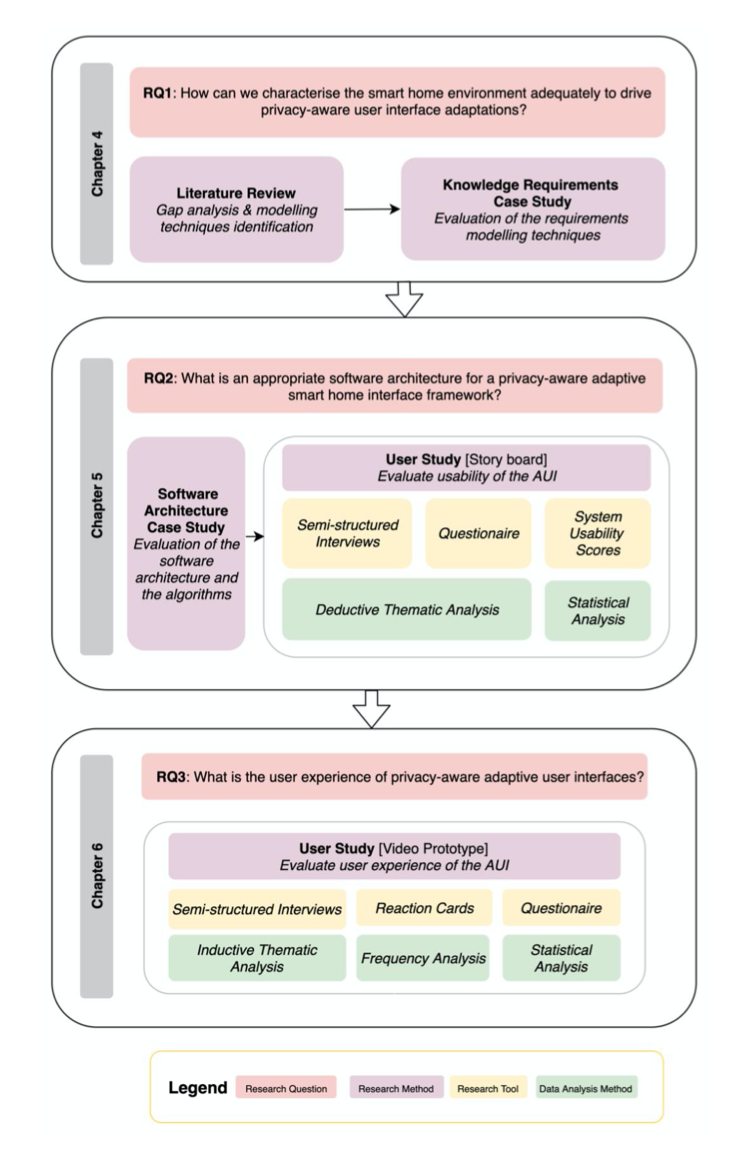
\includegraphics[width=9cm]{images/ephemeral-images-remove-pre-publication/Akshikas-methodology-diagram-from-his-thesis.png}
    \caption{For inspiration only: Akshika's methodologies map}
    \label{fig:akshikas-methodologies-map}
\end{figure}

\hrulefill
\clearpage


The logging case study, in \secref{methodology-map-logging-using-mobile-analytics} uses inductive analysis to determine the patterns. 


\dotfill

\section*{Commentary to address when writing this chapter}
Need to understand what data is actually available that I can collect.
From data to analyses I am undertaking.
In order to get this data 

Therefore I'm going to have to engage with Industry. A case approach, situated in real projects.
How can we generate the evidence and what data can we collect to partially answer the demands for evidence. c.f. data sources section. Provide a foreshadowing of the data sources, signpost to where they will be discussed.

Instantiation in the introduction to the case studies chapter after the model described in the methodology.
Move 5.1 into the methods chapter as it provides orientation for the reader.

I need to decide on my primary organising principle: e.g. the 6 perspectives
Rewrite section 5.1 around figure 5.2 (6 perspectives) Label the 6 perspectives.

In order to understand .... this is what we need, therefore we use the following methods to gather the evidence.

DevEx of the use of the mobile analytics. 

Create a table of the needs to fulfil each of the 6 perspectives: data needed to perspectives i.e. purpose of Analysis, framed in terms of these 6 perspectives. 
Justify how each data source is used to fulfil the research questions. 

From question to evidence to method.

Once the above has been sketched out I can then discuss my roles and I was aware I take different roles and my analysis was cognisant of the different roles I played.

I'd need to define what a case study is. - an opportunity to look in depth in the real world, a container for data collection with and in a number of organisations. I'll explain clearly what methods I was able to use in each case. 

Let me explain in more detail what I mean by... 

*** P1 Start with the table for cases -> types/ categories of data 
*** P2 Table Data types mapped to the analysis I could perform on that data type. What method I used to analyse the data.
Analysis to method may be easier to generate than analysis to purpose.


\section*{Plain thoughts on the methodology used}
Methods need to support real-world projects, their development teams and their apps. Case studies enable this so they were used for the core of the research. Each case study needed the support and agreement of the project team who needed to provide access to the mobile analytics services they use. Those teams and their respective organisations had a bearing on the scope and limits of the research that would be acceptable to them, this meant that case studies were opportunistic in nature and depended on the alignment of purposes, timings, and so on.

There was a fair amount of housekeeping needed to provide and maintain access (where permitted) to the tools. Some teams also allowed access to their bug tracking systems, their source code (and associated build, CI and testing), and - of necessity - their mobile analytics reports. Some wishes aspects of their microcosm to be kept private, in some cases, representative alternatives could be provided that illustrated and/or exemplified some of the learning while maintaining their anonymity.  

Many of the case studies provided extended access to some or all of their systems which enabled some post case study analysis. Learnings from some case studies were able to be used in subsequent ones.

Even though the case studies provided really useful and relevant findings it was clear they did not represent the population of mobile apps. Various Industry contacts who actively use at least one mobile mobile analytics service to monitor failures in their apps agreed to be interviewed and share their insights. Their involvement was approved by their respective projects and/or organisations addressing combined business and ethical perspectives. Again, owing to their specific contexts, concerns, and experiences the interviews were semi-structured to enable them the flexibility, control and freedom to share whatever results, experiences, and insights they were willing and able to provide.

There were some experiments that were not sensible/practical in the case studies; so small scale experiments were designed and performed to research those when it was viable to do so. The ephemeral nature of data and reports in several of the mobile analytics services meant these data and reports were originally hard to record and preserve. The research therefore included the development of software that was able to preserve the data and reports from the core mobile analytics service: Google Play Console with Android Vitals.

Several mobile analytics providers became interested in the research and the results and their perspectives was also of interest and germane to the research, therefore there were symbiotic sharing of results, analysis, product design, customer insights and so on. All these have been anonymised by at least one party and non contained personally identifiable information.  

\newthought{Conceptual Framework}
``Conceptual frameworks provide a theoretical overview of your intended research and order withing that process", ``a map or framework of how the research will be conducted and analysed"~\citep[page 44]{trafford2008_stepping_stones_to_achieving_your_doctorate}

Germane concepts include:
\begin{itemize}
    \item Value Chains and modelling Influences, e.g. see \emph{``From Data to Decisions: A Value Chain for Big Data"}~\citep{miller2013_from_data_to_decisions_a_value_chain_for_big_data} which provides 7 stages in a value chain to obtain value from big data - such as mobile analytics data.
\end{itemize}


The research is mainly empirical owing to the nature of usage analytics and the analytics tools which thrive on volume and realism therefore case studies provide the core of the research. The analytics data for apps is private by default and access is only provided to authorised users of each analytics tool, these users are typically a small trusted subset of the development team for that app. If the development team are part of an organisation they may also need the approval of their organisation before they are permitted to share the analytics outside their immediate team. These restrictions meant an opportunistic approach needed to be taken to obtaining case studies; and the team and/or organisation determined the mode of engagement for the researcher.

Mixed methods were used to expand the research, for instance: by using static analysis into how developers use and maintain remote logging in the codebases of their Android apps, and qualitatively, by interviewing app developers on their use of mobile analytics. 


\isabel{The key concepts and the theoretical framework underpin the methodology: I would say you touch on or assume matters of ontology and the human condition (we are not flawless), management theory (Drucker), systems theory (people, processes and systems interacting), quality models (QiU/Bevan), standards like iso25001 and other models for how we categorise software qualities, psychology (when and how do we trust)}

\newthought{Phrases from Isabel's Transfer Report of relevance} 
A researcher-driven approach using concept maps and influence diagrams to map what I already know from industry experience and previous research. I noticed improving reliability is an ongoing challenge for many software and systems, I focus on Mobile apps and Mobile Analytics for \textit{n} reasons: lastly because I have have extensive experience of developing and improving the quality of mobile apps, `this research is what Aurini [33] characterises as an \textit{of me} research problem, that is, whilst I am the researcher, I could also be a participant.' It also includes a \textit{plus 1} research project, as it adds to the current research on practitioner practices and experiences... An empirical approach to data collection and analysis. 
%
Clough and Nutbrown’s approach to research methodology [1] includes an imperative that research is both political and persuasive, with the intent of influencing strategy and approaches in working practices (see Figure 2, page 7). In their case, they apply this to research into and affecting social policy, however I feel the same purpose is important with regard to the politics, policies, strategies and approaches to testing used in organisations and their IT teams. As an industry practitioner coming into academia, I am in a position to learn from and potentially to influence both industry and academia, working on ICT, SWT and other disciplines, bridging research and industry practice.
%
Groups contributing to and receiving information about results...
%
My results report on the practitioners' reality.

\newthought{Case Studies}
The case studies illustrate manifold facets of applying (and ignoring) mobile analytics across various contexts of engagement, across various types of app, and from several perspectives including the organizations who create the mobile analytics tools and related services.

The case studies include examples where the researcher's mode of engagement was as:
\begin{enumerate}
    \itemsep0em
    \item an embedded developer: an active participant integrated into the project team,
    \item a coach: of an existing team of developers who applied the concepts,
    \item an interviewer: of various development teams to learn of their practices and results,
    \item an analyst/observer: performing static analysis of opensource code repositories.
\end{enumerate}
\isabel{I think if you look at this in terms of the methodology, you can weave in some of the things Aurini, Heath, and Howells talk about. So in the first two points the research is "of me" whereas in points 3 and 4 it is not. From Clough and Nutbrown, in points 1 and 2 the way you can be political and persuasive is different to how you apply political/persuasive as a result of 3 and 4. When you are a coach the point of being in the project is to effect change. The research effects change as a result of how you promulgate the results}

Research effecting change when I am an active part of it, i.e. in 1 and 2 above.




\begin{figure}
    \centering
    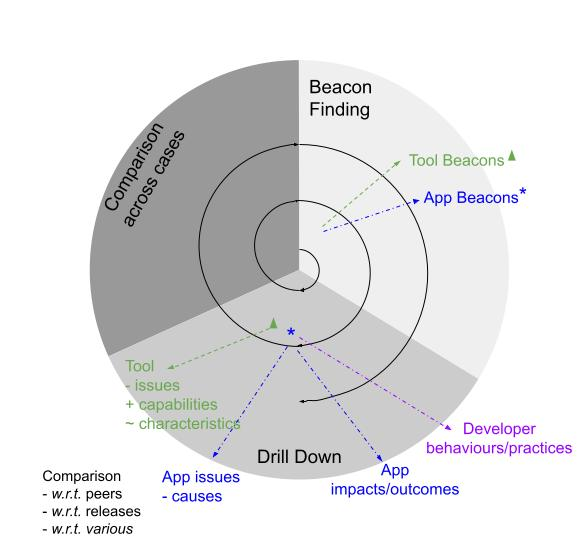
\includegraphics[width=14cm]{images/my/Illustrated-Research-Methodology-using-Mobile-Analytics-as-the-Epicentre-v0-2.jpeg}
    \caption{Illustrated Research Methodology using Mobile-Analytics as the Epicentre [TODO Revise]}
    \label{fig:Illustrated-Research-Methodology-using-Mobile-Analytics-as-the-Epicentre}
\end{figure}

The first representation of the iterative cycle is illustrated in Figure~\ref{fig:Illustrated-Research-Methodology-using-Mobile-Analytics-as-the-Epicentre}. This shows an artificially clean and orderly progression between elements in the cycle and useful to communicate the concepts of the research methodology. 

However this Figure (\ref{fig:Illustrated-Research-Methodology-using-Mobile-Analytics-as-the-Epicentre}) does not incorporate real-world and practical characteristics of app development practice, which is the crucible for this research.